\documentclass{beamer-control}
\usepackage{beamer-control-singlefile}
\INCLUDEONLY{Frequency Domain Modeling}
\begin{document}
\CONCEPT{Frequency Domain Modeling}

\begin{SUMMARY}
\begin{itemize}
\item Comparison of state space and transfer function approaches
\item Standardised block diagram of a transfer-function centric control system
\end{itemize}
\vfill References:
\begin{itemize}
\item \astrom{§9.1}
\end{itemize}
\end{SUMMARY}


\begin{frame}
\frametitle{Transfer Functions}
\framesubtitle{A different approach to state space}

\begin{itemize}
\item State Space modelling starts with ODEs and allows highly structured approaches to represent MIMO linear and nonlinear systems
\item Transfer Function modelling is a more classical approach
\begin{itemize}
\item Assumes linear systems (mostly)
\item Can only consider SISO systems
\item Uses frequency domain representation instead of ODEs directly
\item Mathematically simpler
\end{itemize}
\end{itemize}

\end{frame}

\begin{frame}
\frametitle{Frequency domain --- periodic input signals}

Consider periodic input signal $u(t)$. Can be represented as:
\begin{align}
u(t) = \sum_{k=0}^\infty\left\{ a_k \sin k\omega_f t + b_k \cos k \omega_f t \right\}
\end{align}
where $\omega_f$ is the \emph{fundamental frequency} of the periodic input (i.e., $\tfrac{2\pi}{T_f}$ where $T_f$ is the time span of one period)

\bigskip
\begin{uncoverenv}<2->
\alert{Because of linearity \& superposition, we can consider each frequency independently and `add up' the solutions for each}
\end{uncoverenv}
\end{frame}

\begin{frame}
\frametitle{Frequency domain --- single frequency}
\begin{itemize}
\item We have sinusoidal input $u(t)$ and sinusoidal output $y(t)$
\item Gain $M$ and phase $\theta$ from input to output given at each frequency $\ww$ by
\begin{align}
G(\ii\ww) &= C(\ii\ww I - A)^{-1}B + D = M\ee^{\ii\theta}
\end{align}
where we set $\ww=k \omega_f$ for $k=1,2,\dots$
\item See topic 3.4 / \AMref{§6.3}
\item \alert{This equation generalises for complex exponential inputs as well: $u(t) = \ee^{st}$:
\begin{align}
G(s) &= C(s I - A)^{-1}B + D = M\ee^{\ii\theta}
\end{align}
}
\end{itemize}

\end{frame}

\begin{frame}
\frametitle{}
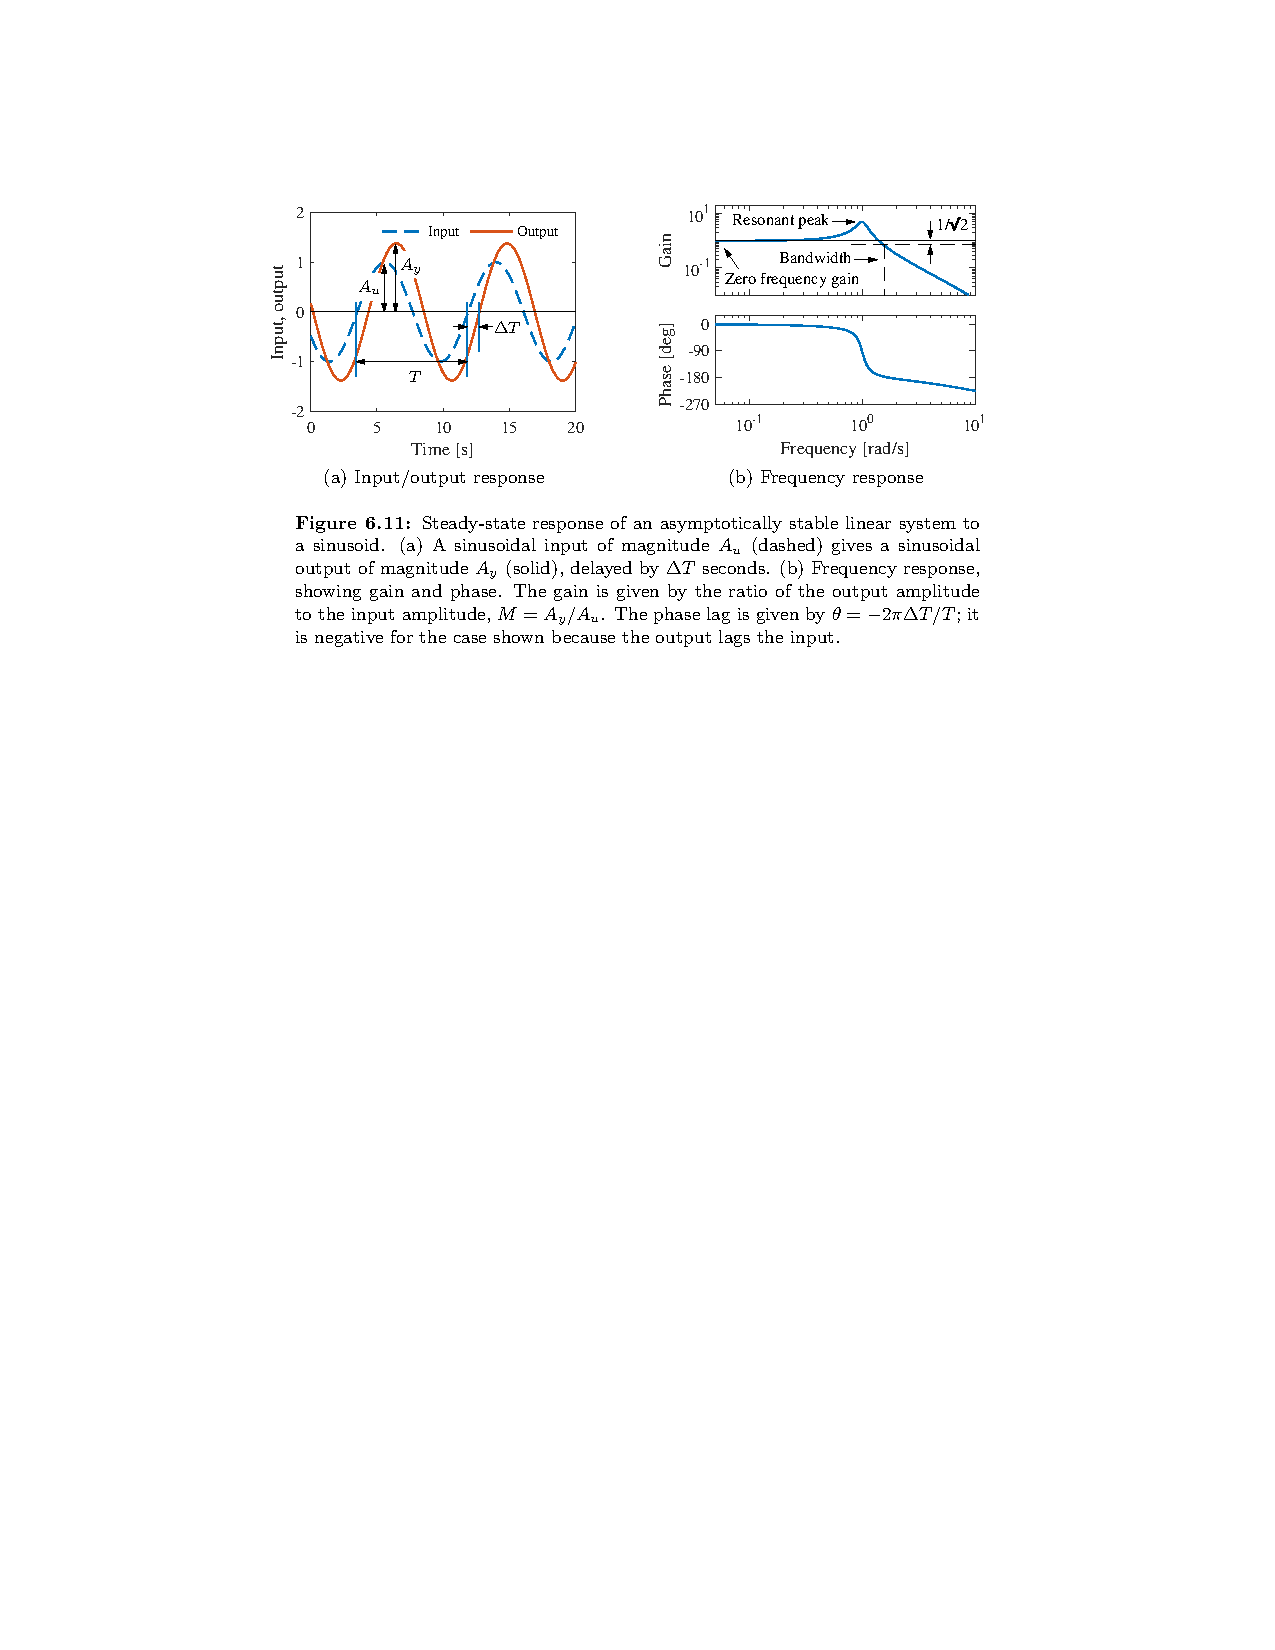
\includegraphics[width=\linewidth]{figure6.11}

\end{frame}

\begin{frame}
\frametitle{Frequency response advantages}

\begin{itemize}
\item Strong conceptual basis for modelling systems
\item Graphical approaches to plotting and comparing system response
\item Powerful yet simple approach to analyse system stability
\item Intuitive measures for considering performance and robustness
\item Natural extension to consider disturbances and measurement noise
\end{itemize}

\end{frame}

\begin{frame}
\frametitle{Block diagram}

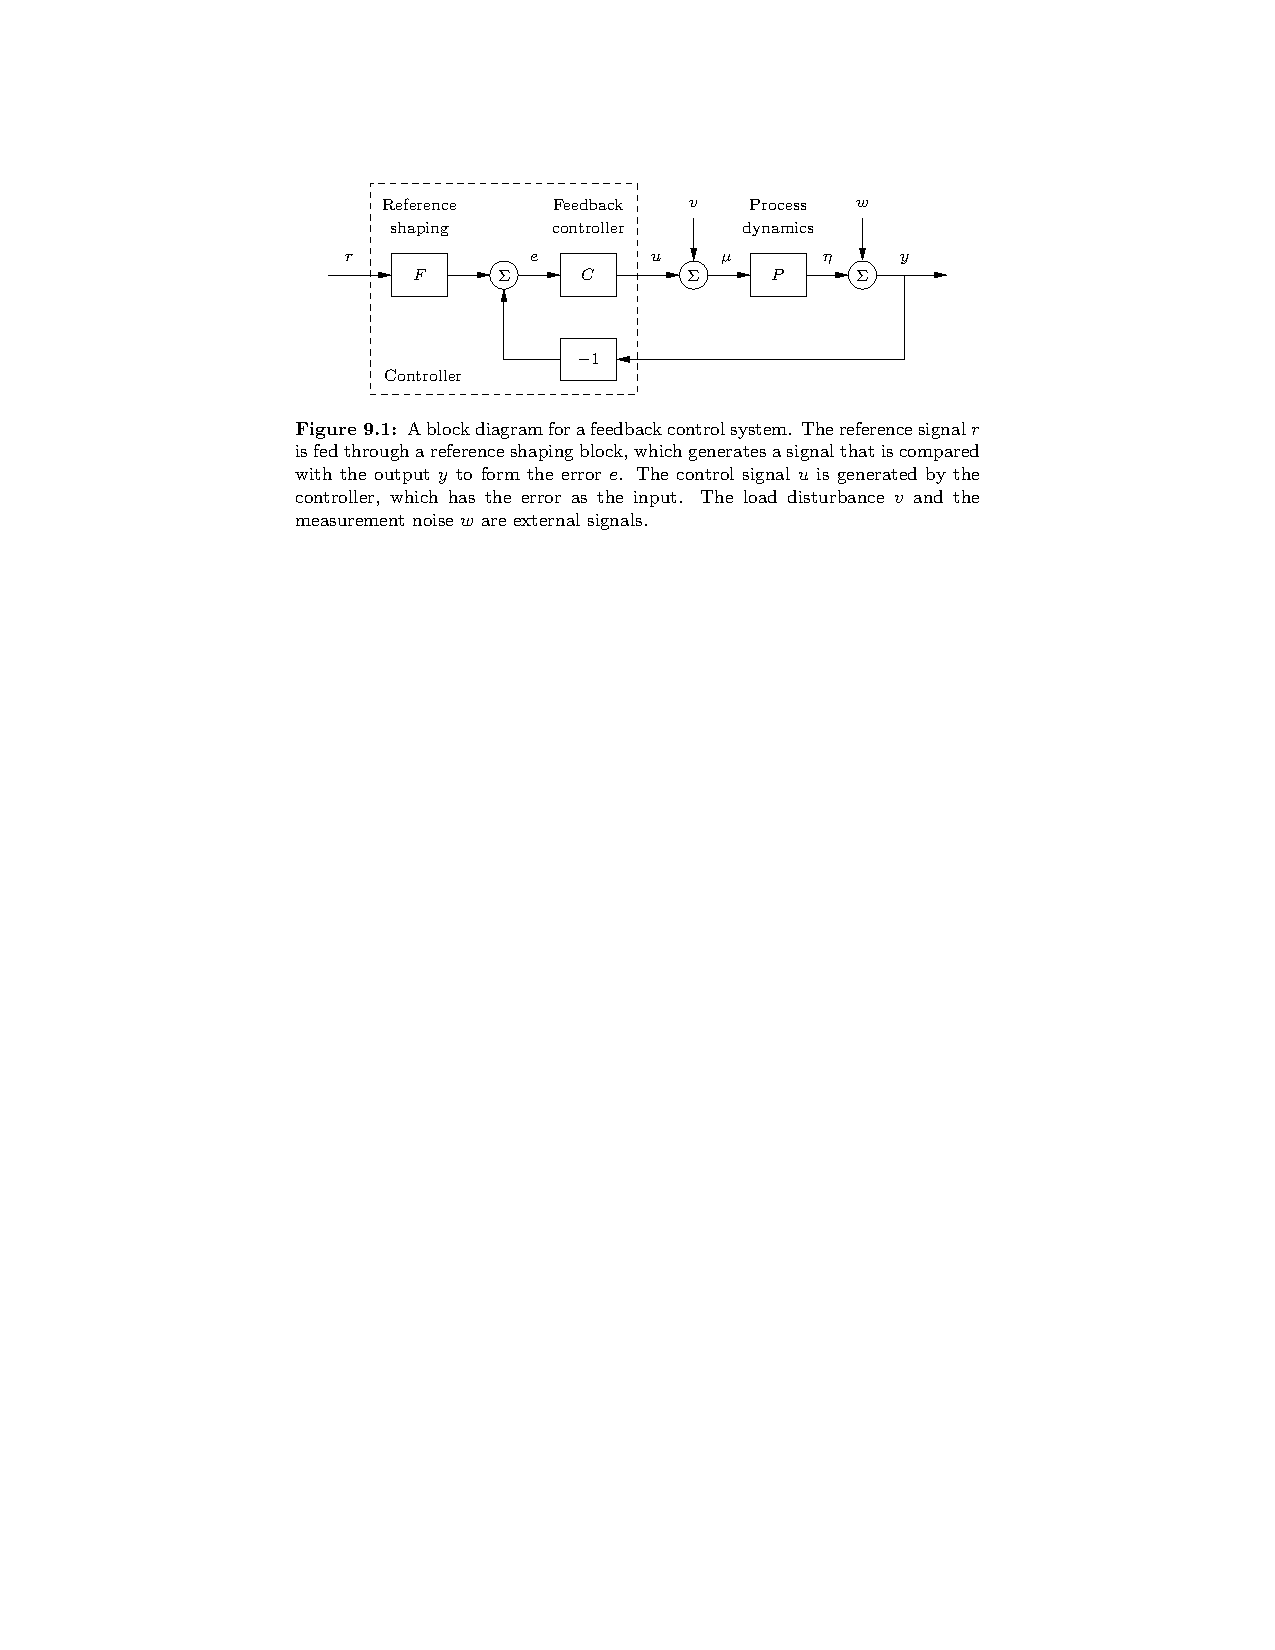
\includegraphics[width=\linewidth]{figure9.1}


\end{frame}

\begin{frame}
\frametitle{Block diagram features}
\begin{itemize}
\item Reference input $r$
\item Reference shaping $F$
\item Feedback controller $C$
\item Disturbance input $v$
\item Process dynamics $P$
\item Measurement noise $w$
\item Output $y$
\end{itemize}
\end{frame}



\SUMMARYFRAME
\FINALE

\end{document}
